\NeedsTeXFormat{LaTeX2e}
%\PassOptionsToClass{handout}{beamer}
\documentclass{beamer}
\usepackage{beamerPack}
\usepackage[boxed,ruled,vlined]{algorithm2e}
\usepackage{setspace}
\usepackage[usestackEOL]{stackengine}[2013-10-15]
\def\x{\hspace{4.1ex}}    %BETWEEN TWO 1-DIGIT NUMBERS
\def\y{\hspace{3.4ex}}  %BETWEEN 1 AND 2 DIGIT NUMBERS
\def\z{\hspace{2.7ex}}    %BETWEEN TWO 2-DIGIT NUMBERS
\usetikzlibrary{arrows.meta}
\usepackage[04]{../lecture}
\subtitle{練習問題}
\begin{document}

\begin{frame}[fragile]{}
\titlepage
\end{frame}

\section{Algorithm design}		%%%%%%%%
\subsection{}

\begin{frame}[fragile]{問題解決の枠組み}{}
\begin{enumerate}\itemsep8pt
\item 問題の解法をアルゴリズム化する
\begin{align*}
アルゴリズム = & 前処理? 相似問題^{+} 後処理?
\end{align*}
\item (要求を満たすまで無駄を省く)
\item プログラムとして実装する
\item (要求を満たすまで高速化する)
\end{enumerate}
\end{frame}

\begin{frame}[fragile]{アルゴリズムでは再帰であること}{}
fact(100), Fib(100), A(3, 3)を求めるプログラムを作成せよ
\begin{align*}
fact(1) =& 1 \\
fact(n) =& n \times fact(n - 1)\\
Fib(1) =& 1 \\
Fib(2) =& 1 \\
Fib(n) =& Fib(n - 1) + Fib(n -2) \\
A(0, n) =& n + 1 \\
A(m, 0) =& A(m - 1, 1) \\
A(m, n) =& A(m - 1, A(m, n - 1))
\end{align*}

\begin{itemize}%\itemsep8pt
\item $f(n) = ? + f(-) + ?$ :: 線形再帰
\item $f(n) = ? + f(-)$ :: 線形再帰、特に末尾再帰\href{https://ja.wikipedia.org/wiki/%E6%9C%AB%E5%B0%BE%E5%86%8D%E5%B8%B0}{\beamergotobutton{wikipedia}}
\item $f(n) = ? + f(-) + f(-) + ?$ :: 線形再帰でない
\end{itemize}
\end{frame}

\section{A series of practices}		%%%%%%%%
\subsection{}

\begin{frame}[fragile]{問題0.0}{}
\stackMath
\Longstack[l]{
n=0\\
n=1\\
n=2\\
n=3\\
n=4\\
n=5\\
n=6\\
n=7\qquad\ \\
}
\Longstack{
1\\
1\x 1\\
1\x 2\x 1\\
1\x 3\x 3\x 1\\
1\x 4\x 6\x 4\x 1\\
1\x 5\y 10\z 10\y 5\x 1\\
1\x 6\y 15\z 20\z 15\y 6\x 1\\
1\x 7\x 21\z 35\z 35\z 21\y 7\x 1\\
}

$n = 23$, 左から11番目の数は?
\end{frame}

\begin{frame}[fragile]{構造}{}
\visible<2->{
\begin{align*}
P(-) &= P(北東) + P(北西)
\end{align*}
}
\begin{center}
\rotatebox{-45}{
\scalebox{0.6}{
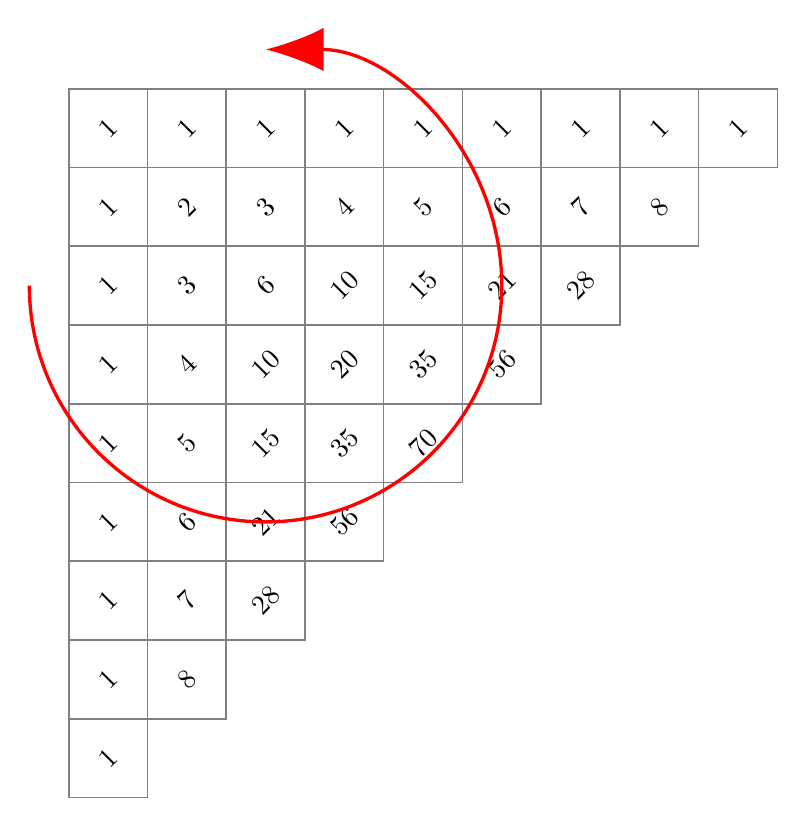
\begin{tikzpicture}[cell/.style = {rectangle,draw=gray,semithick,minimum size=1cm,outer sep=0mm}]
\foreach \i [count=\j from 0] in {1, 1, 1, 1, 1,  1, 1, 1, 1}
    \node[cell] at (\j,  0) {\rotatebox{45}{$\i$}};
\foreach \i [count=\j from 0] in {1, 2, 3, 4, 5,  6, 7, 8}
    \node[cell] at (\j, -1) {\rotatebox{45}{$\i$}};
\foreach \i [count=\j from 0] in {1, 3, 6, 10,15,21,28}
    \node[cell] at (\j, -2) {\rotatebox{45}{$\i$}};
\foreach \i [count=\j from 0] in {1, 4, 10,20,35,56}
    \node[cell] at (\j, -3) {\rotatebox{45}{$\i$}};
\foreach \i [count=\j from 0] in {1, 5, 15,35,70}
    \node[cell] at (\j, -4) {\rotatebox{45}{$\i$}};
\foreach \i [count=\j from 0] in {1, 6, 21,56}
    \node[cell] at (\j, -5) {\rotatebox{45}{$\i$}};
\foreach \i [count=\j from 0] in {1, 7, 28}
    \node[cell] at (\j, -6) {\rotatebox{45}{$\i$}};
\foreach \i [count=\j from 0] in {1, 8}
    \node[cell] at (\j, -7) {\rotatebox{45}{$\i$}};
\foreach \i [count=\j from 0] in {1}
    \node[cell] at (\j, -8) {\rotatebox{45}{$\i$}};
\visible<3>{\draw[-{Latex[scale=2.5]},red, very thick] (-1,-2) arc (180:450:3);}
\end{tikzpicture}
}
}
\end{center}
\end{frame}

\begin{frame}[fragile]{イメージしやすい形に回転(変数変換)}{}
\begin{center}
\scalebox{0.5}{
\begin{tikzpicture}[cell/.style = {rectangle,draw=gray,semithick,minimum size=1cm,outer sep=0mm}]
\foreach \i [count=\j from 0] in {1, 1, 1, 1, 1,  1, 1, 1, 1}
    \node[cell] at (\j, 0) {\rotatebox{0}{$\i$}};
\foreach \i [count=\j from 0] in {1, 2, 3, 4, 5,  6, 7, 8}
    \node[cell] at (\j, 1) {\rotatebox{0}{$\i$}};
\foreach \i [count=\j from 0] in {1, 3, 6, 10,15,21,28}
    \node[cell] at (\j, 2) {\rotatebox{0}{$\i$}};
\foreach \i [count=\j from 0] in {1, 4, 10,20,35,56}
    \node[cell] at (\j, 3) {\rotatebox{0}{$\i$}};
\foreach \i [count=\j from 0] in {1, 5, 15,35,70}
    \node[cell] at (\j, 4) {\rotatebox{0}{$\i$}};
\foreach \i [count=\j from 0] in {1, 6, 21,56}
    \node[cell] at (\j, 5) {\rotatebox{0}{$\i$}};
\foreach \i [count=\j from 0] in {1, 7, 28}
    \node[cell] at (\j, 6) {\rotatebox{0}{$\i$}};
\foreach \i [count=\j from 0] in {1, 8}
    \node[cell] at (\j, 7) {\rotatebox{0}{$\i$}};
\foreach \i [count=\j from 0] in {1}
    \node[cell] at (\j, 8) {\rotatebox{0}{$\i$}};
\draw[arrow] (0, -1) -- ++(10, 0) node[below] {N=23 (X=23)};
\draw[arrow] (-1, 0) -- ++(0, 10) node[left] {Y};
\draw[arrow] (10, 0) -- ++ (-6, 6) node[right=5pt, anchor=west] {左から11(10回移動)};
\end{tikzpicture}
}
\end{center}
求める場所は座標$(13, 10)$に対応
\end{frame}

\begin{frame}[fragile]{配列の是非}{}

与えられた問題は点(13, 10)を求める

大きさ(13,10)の表を完成させる問題を解けば簡単に求められる

\vfill
\begin{itemize}\itemsep8pt
\item ゴールから遡ると再帰関数が必要(補助記憶領域なし)
\item (帰納的構造を理解した上で)スタートから組み立てると配列が必要(再帰なし)
\end{itemize}

\vfill
「配列を使ってはいけない」という追加制約があっても解けるのならOK

\vfill
{\fontsize{5}{5}\selectfont ただし電卓問題ではスタートからの組み立ては無理}
\end{frame}

\begin{frame}[fragile]{問題1.0}{}
\begin{tikzpicture}[overlay, xshift=0.5\textwidth,yshift=-0.25\textheight]
\node at (0,0) {\pgfimage[width=1.0\pagewidth]{shuttle.jpg}};
\end{tikzpicture}
\begin{spacing}{1.25}
\textcolor{white}{
観光用スペースシャトルが高度100キロメートルからツアーを開始します。\\
乗客は1分ごとに次の1分間上昇するか、下降するかを決めることができます。どちらも1分でちょうど1キロ上昇するか下降します。\\
30分後(30回の進路変更後)に元の高度に戻ってこなければならないとすると、飛行経路は何通りあるでしょう。
}
\end{spacing}
\end{frame}

\begin{frame}[fragile]{}{}
\begin{tikzpicture}[overlay , xshift=0.5\textwidth]
\visible<1>{\node[anchor=west] at (0, -5) {30で元の高さ};}
\visible<2>{\node[anchor=west] at (1, -5) {30で元の高さ $\to$ 座標(15,15)};}
\end{tikzpicture}

\begin{center}
\rotatebox{45}{
\scalebox{0.4}{
\begin{tikzpicture}[cell/.style = {rectangle,draw=gray,semithick,minimum size=1cm,outer sep=0mm}]
\foreach \i [count=\j from 0] in {1, 1, 1, 1, 1,  1, 1, 1, 1}
    \node[cell] at (\j,  0) {\rotatebox{-45}{$\i$}};
\foreach \i [count=\j from 0] in {1, 2, 3, 4, 5,  6, 7, 8}
    \node[cell] at (\j, -1) {\rotatebox{-45}{$\i$}};
\foreach \i [count=\j from 0] in {1, 3, 6, 10,15,21,28}
    \node[cell] at (\j, -2) {\rotatebox{-45}{$\i$}};
\foreach \i [count=\j from 0] in {1, 4, 10,20,35,56}
    \node[cell] at (\j, -3) {\rotatebox{-45}{$\i$}};
\foreach \i [count=\j from 0] in {1, 5, 15,35,70}
    \node[cell] at (\j, -4) {\rotatebox{-45}{$\i$}};
\foreach \i [count=\j from 0] in {1, 6, 21,56}
    \node[cell] at (\j, -5) {\rotatebox{-45}{$\i$}};
\foreach \i [count=\j from 0] in {1, 7, 28}
    \node[cell] at (\j, -6) {\rotatebox{-45}{$\i$}};
\foreach \i [count=\j from 0] in {1, 8}
    \node[cell] at (\j, -7) {\rotatebox{-45}{$\i$}};
\foreach \i [count=\j from 0] in {1}
    \node[cell] at (\j, -8) {\rotatebox{-45}{$\i$}};
\node[fill=red] at (10,-10) {\rotatebox{-45}{\textcolor{red}{\textcolor{white}{ゴール}}}};
\draw[draw=black,-{Latex[scale=2]}] (-0.5, 0.5) -- ++(12, 0);
\draw[draw=black,-{Latex[scale=2]}] (-0.5, 0.5) -- ++(0, -12);
\draw[-{Latex[scale=1.5]}] (-3, -1) -- (-0.5, 0);
\node[rotate=-45] at (-3.5,-1.8) {原点$(0,0)$};
\end{tikzpicture}
}
}
\end{center}

\end{frame}

\begin{frame}[fragile]{問題1.1}{}
\begin{tikzpicture}[overlay, xshift=0.5\textwidth,yshift=-0.22\textheight]
\node at (0,-1) {\pgfimage[width=0.5\pagewidth]{smalltalk.jpg}};
\end{tikzpicture}

\begin{spacing}{1.25}
観光用飛行船が高度5キロメートルからツアーを開始します。\\
乗客は1分ごとに次の1分間上昇するか、下降するかを決めることができます。どちらも1分でちょうど1キロ上昇するか下降します。\\
30分後(30回の進路変更後)に元の高度に戻ってこなければならないとすると、飛行経路は何通りあるでしょう。\\
高度0キロメートルで墜落します。
\end{spacing}

\end{frame}

\begin{frame}[fragile]{}{}
\begin{center}
\rotatebox{45}{
\scalebox{0.5}{
\begin{tikzpicture}[cell/.style = {rectangle,draw=gray,semithick,minimum size=1cm,outer sep=0mm}]
\foreach \i [count=\j from 0] in {1, 1, 1, 1, 1, 1, 1, 1, 1}
    \node[cell] at (\j,  0) {\rotatebox{-45}{$\i$}};
\foreach \i [count=\j from 0] in {1, 2, 3, 4, 5,  6, 7, 8}
    \node[cell] at (\j, -1) {\rotatebox{-45}{$\i$}};
\foreach \i [count=\j from 0] in {1, 3, 6, 10,15,21,28}
    \node[cell] at (\j, -2) {\rotatebox{-45}{$\i$}};
\foreach \i [count=\j from 0] in {1, 4, 10,20,35,56}
    \node[cell] at (\j, -3) {\rotatebox{-45}{$\i$}};
\foreach \i [count=\j from 0] in {1, 5, 15, 35, 70}
    \node[cell] at (\j, -4) {\rotatebox{-45}{$\i$}};
\foreach \i [count=\j from 0] in {X, 6, 21, 56}
    \node[cell] at (\j, -5) {\rotatebox{-45}{$\i$}};
\foreach \i [count=\j from 0] in {X, X, 28}
    \node[cell] at (\j, -6) {\rotatebox{-45}{$\i$}};
\foreach \i [count=\j from 0] in {X, X}
    \node[cell] at (\j, -7) {\rotatebox{-45}{$\i$}};
\foreach \i [count=\j from 0] in {X}
    \node[cell] at (\j, -8) {\rotatebox{-45}{$\i$}};
\draw[draw=red,rotate=-45,very thick] (1,-3.5) -- ++(10,0) node[rotate=-45,above=4pt] () {地平線};
\end{tikzpicture}
}
}
\end{center}
\end{frame}

\begin{frame}[fragile]{回転}{}
\begin{center}
\scalebox{0.5}{
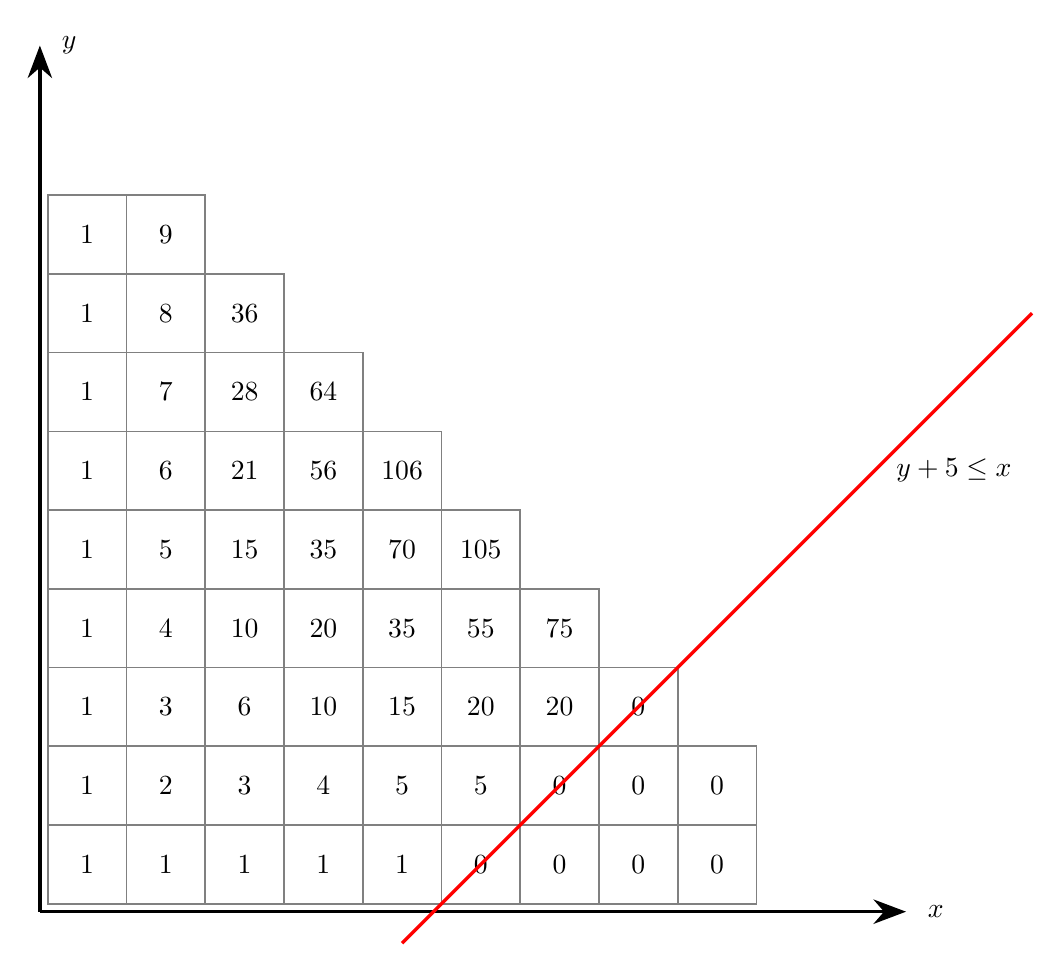
\begin{tikzpicture}[cell/.style = {rectangle,draw=gray,semithick,minimum size=1cm,outer sep=0mm}]
\foreach \i [count=\j from 0] in {1, 1, 1, 1, 1, 0, 0, 0, 0}
    \node[cell] at (\j,  0) {\rotatebox{0}{$\i$}};
\foreach \i [count=\j from 0] in {1, 2, 3, 4, 5, 5, 0, 0, 0}
    \node[cell] at (\j, 1) {\rotatebox{0}{$\i$}};
\foreach \i [count=\j from 0] in {1, 3, 6, 10,15,20, 20, 0}
    \node[cell] at (\j, 2) {\rotatebox{0}{$\i$}};
\foreach \i [count=\j from 0] in {1, 4, 10,20,35,55, 75}
    \node[cell] at (\j, 3) {\rotatebox{0}{$\i$}};
\foreach \i [count=\j from 0] in {1, 5, 15, 35, 70, 105}
    \node[cell] at (\j, 4) {\rotatebox{0}{$\i$}};
\foreach \i [count=\j from 0] in {1, 6, 21, 56, 106}
    \node[cell] at (\j, 5) {\rotatebox{0}{$\i$}};
\foreach \i [count=\j from 0] in {1, 7, 28, 64}
    \node[cell] at (\j, 6) {\rotatebox{0}{$\i$}};
\foreach \i [count=\j from 0] in {1, 8, 36}
    \node[cell] at (\j, 7) {\rotatebox{0}{$\i$}};
\foreach \i [count=\j from 0] in {1, 9}
    \node[cell] at (\j, 8) {\rotatebox{0}{$\i$}};
\draw[-{Stealth[scale=1.4]},draw=black,very thick] (-0.6,-0.6) -- ++(11,0) node[right=4pt] {$x$};
\draw[-{Stealth[scale=1.4]},draw=black,very thick] (-0.6,-0.6) -- ++(0,11) node[right=4pt] {$y$};
\draw[draw=red,very thick] (4,-1) -- ++(8,8) node[near end, right=4pt] () {$y + 5 \le x$};
\end{tikzpicture}
}
\end{center}
\end{frame}

\begin{frame}[fragile]{問題1.2}{}
あなたはAブロックでお客を拾ったタクシードライバーです。お客はBブロックに行こうとしています。
リアルタイム混雑情報サービスはブロック内移動時間を以下のように表示しています。
最短で何分あればBブロックに到着できるでしょう。
どのブロックも下から上または左から右へ一方通行でつながっています。

\begin{center}
\scalebox{0.25}{
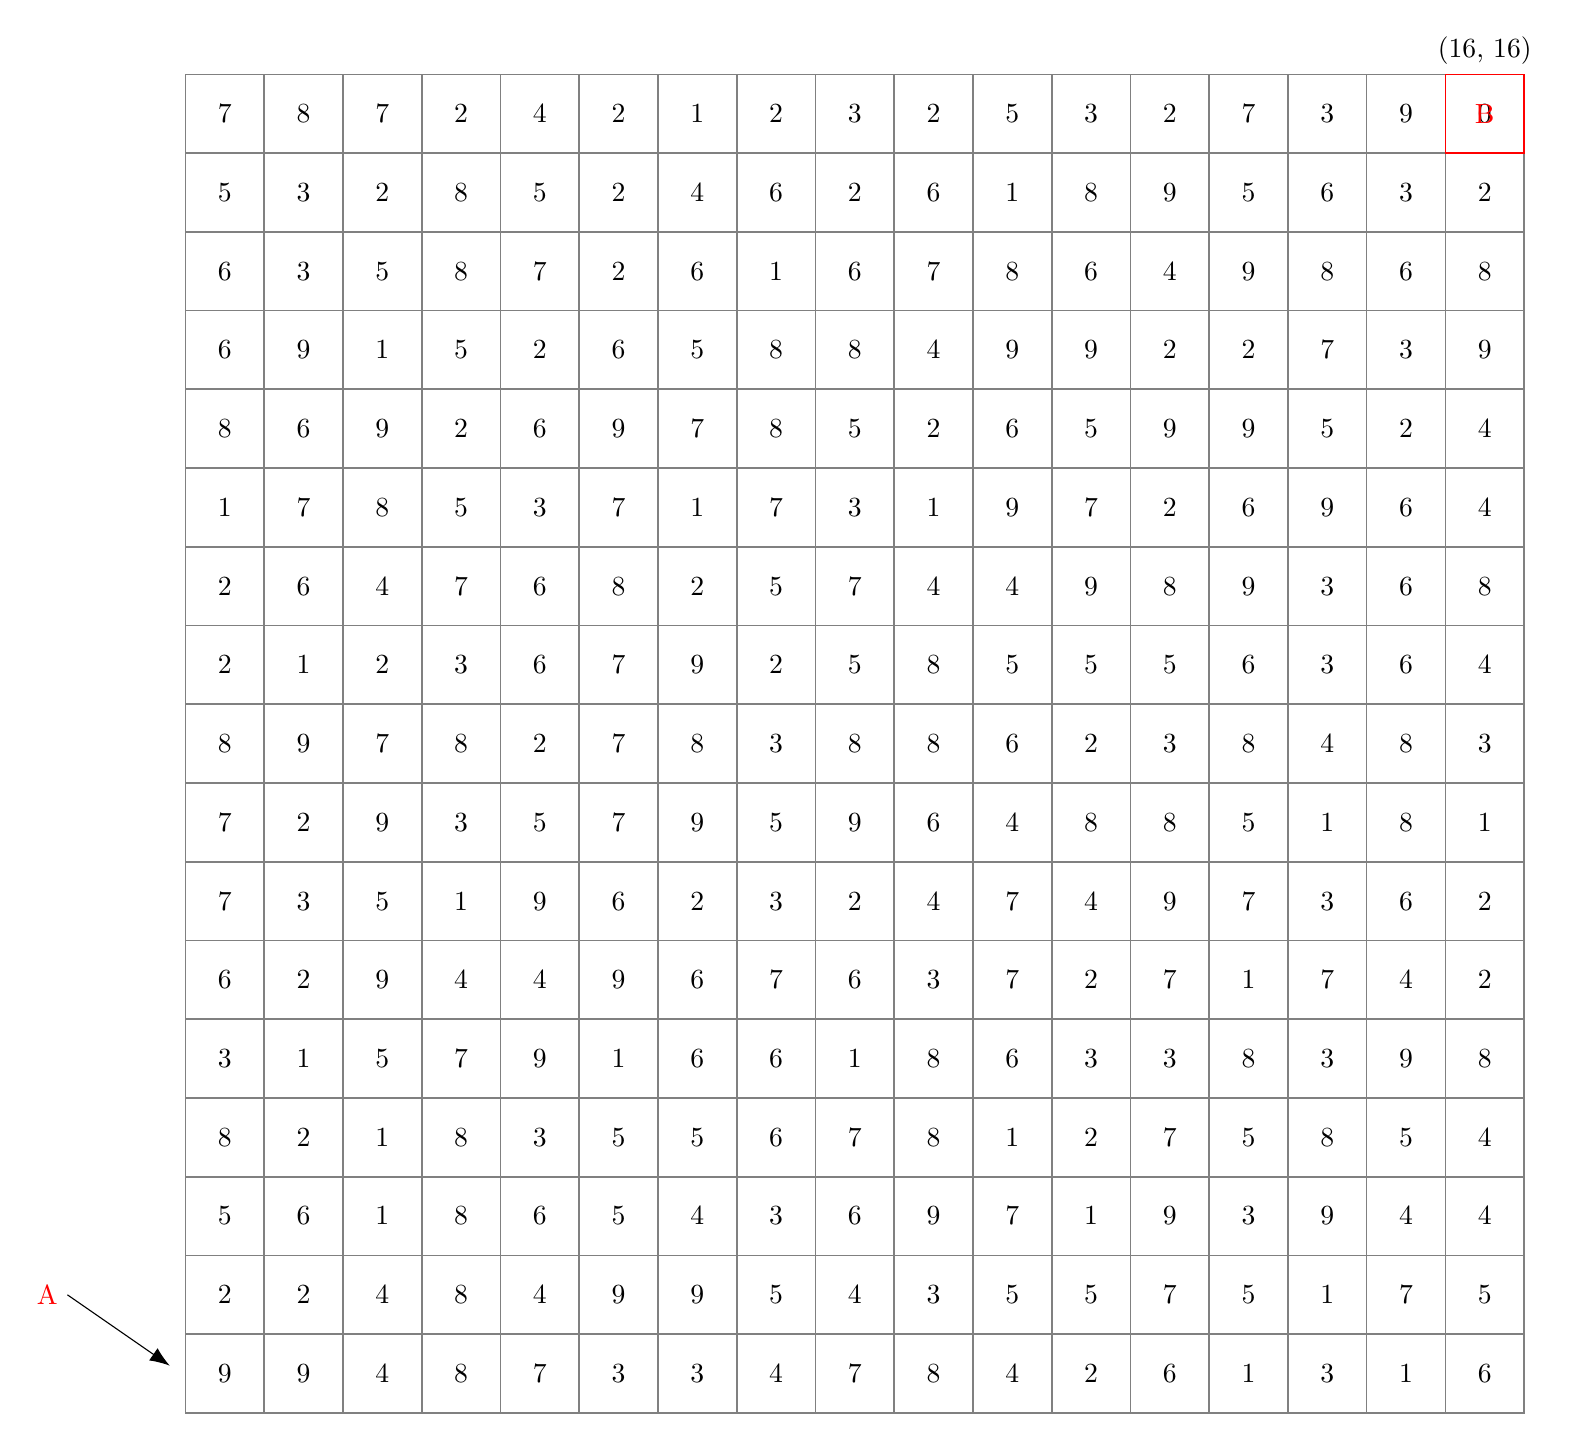
\begin{tikzpicture}[cell/.style = {rectangle,draw=gray,semithick,minimum size=1cm,outer sep=0mm}]
    \foreach \i [count=\j from 0] in {9,9,4,8,7,3,3,4,7,8,4,2,6,1,3,1,6} \node[cell] at (\j, 0) {$\i$};
    \foreach \i [count=\j from 0] in {2,2,4,8,4,9,9,5,4,3,5,5,7,5,1,7,5} \node[cell] at (\j, 1) {$\i$};
    \foreach \i [count=\j from 0] in {5,6,1,8,6,5,4,3,6,9,7,1,9,3,9,4,4} \node[cell] at (\j, 2) {$\i$};
    \foreach \i [count=\j from 0] in {8,2,1,8,3,5,5,6,7,8,1,2,7,5,8,5,4} \node[cell] at (\j, 3) {$\i$};
    \foreach \i [count=\j from 0] in {3,1,5,7,9,1,6,6,1,8,6,3,3,8,3,9,8} \node[cell] at (\j, 4) {$\i$};
    \foreach \i [count=\j from 0] in {6,2,9,4,4,9,6,7,6,3,7,2,7,1,7,4,2} \node[cell] at (\j, 5) {$\i$};
    \foreach \i [count=\j from 0] in {7,3,5,1,9,6,2,3,2,4,7,4,9,7,3,6,2} \node[cell] at (\j, 6) {$\i$};
    \foreach \i [count=\j from 0] in {7,2,9,3,5,7,9,5,9,6,4,8,8,5,1,8,1} \node[cell] at (\j, 7) {$\i$};
    \foreach \i [count=\j from 0] in {8,9,7,8,2,7,8,3,8,8,6,2,3,8,4,8,3} \node[cell] at (\j, 8) {$\i$};
    \foreach \i [count=\j from 0] in {2,1,2,3,6,7,9,2,5,8,5,5,5,6,3,6,4} \node[cell] at (\j, 9) {$\i$};
    \foreach \i [count=\j from 0] in {2,6,4,7,6,8,2,5,7,4,4,9,8,9,3,6,8} \node[cell] at (\j, 10) {$\i$};
    \foreach \i [count=\j from 0] in {1,7,8,5,3,7,1,7,3,1,9,7,2,6,9,6,4} \node[cell] at (\j, 11) {$\i$};
    \foreach \i [count=\j from 0] in {8,6,9,2,6,9,7,8,5,2,6,5,9,9,5,2,4} \node[cell] at (\j, 12) {$\i$};
    \foreach \i [count=\j from 0] in {6,9,1,5,2,6,5,8,8,4,9,9,2,2,7,3,9} \node[cell] at (\j, 13) {$\i$};
    \foreach \i [count=\j from 0] in {6,3,5,8,7,2,6,1,6,7,8,6,4,9,8,6,8} \node[cell] at (\j, 14) {$\i$};
    \foreach \i [count=\j from 0] in {5,3,2,8,5,2,4,6,2,6,1,8,9,5,6,3,2} \node[cell] at (\j, 15) {$\i$};
    \foreach \i [count=\j from 0] in {7,8,7,2,4,2,1,2,3,2,5,3,2,7,3,9,0} \node[cell] at (\j, 16) {$\i$};
\draw[{Latex[scale=1.5]}-] (-0.7, 0.1) -- (-2,1) node[left] {\textcolor{red}{A}};
\node[cell,red,label={(16, 16)}] at (16,16) {B};
\end{tikzpicture}
}
\end{center}
\end{frame}

\begin{frame}[fragile]{配布ファイル}{toa04-p1.2-routes.txt}
\begin{codeof}{language=c}{Y, X = N}
 0, 0 = 9
 0, 1 = 9
 0, 2 = 4
 0, 3 = 8
 0, 4 = 7
...
 1, 0 = 2
 1, 1 = 2
 1, 2 = 4
 1, 3 = 8
...
 2, 0 = 5
\end{codeof}

1行目の意味:座標$(0, 0)$のブロックを(どの方向であれ)通り抜けるには9分かかる。
従って座標$(1,0)$のブロックにたどり着くには9分が必要。座標$(0,1)$も同様に9分。
\end{frame}


\begin{frame}[fragile]{問題1.2.1}{}
あなたはAブロックでお客を拾ったタクシードライバーです。お客はBブロックに行こうとしています。
RCISはそれぞれのブロック内移動時間を以下のように表示しています。
最短で何分あればBブロックに到着できるでしょう。
どのブロックも下から上、左から右、または左下から右上へ一方通行でつながっています。

\begin{center}
\scalebox{0.25}{
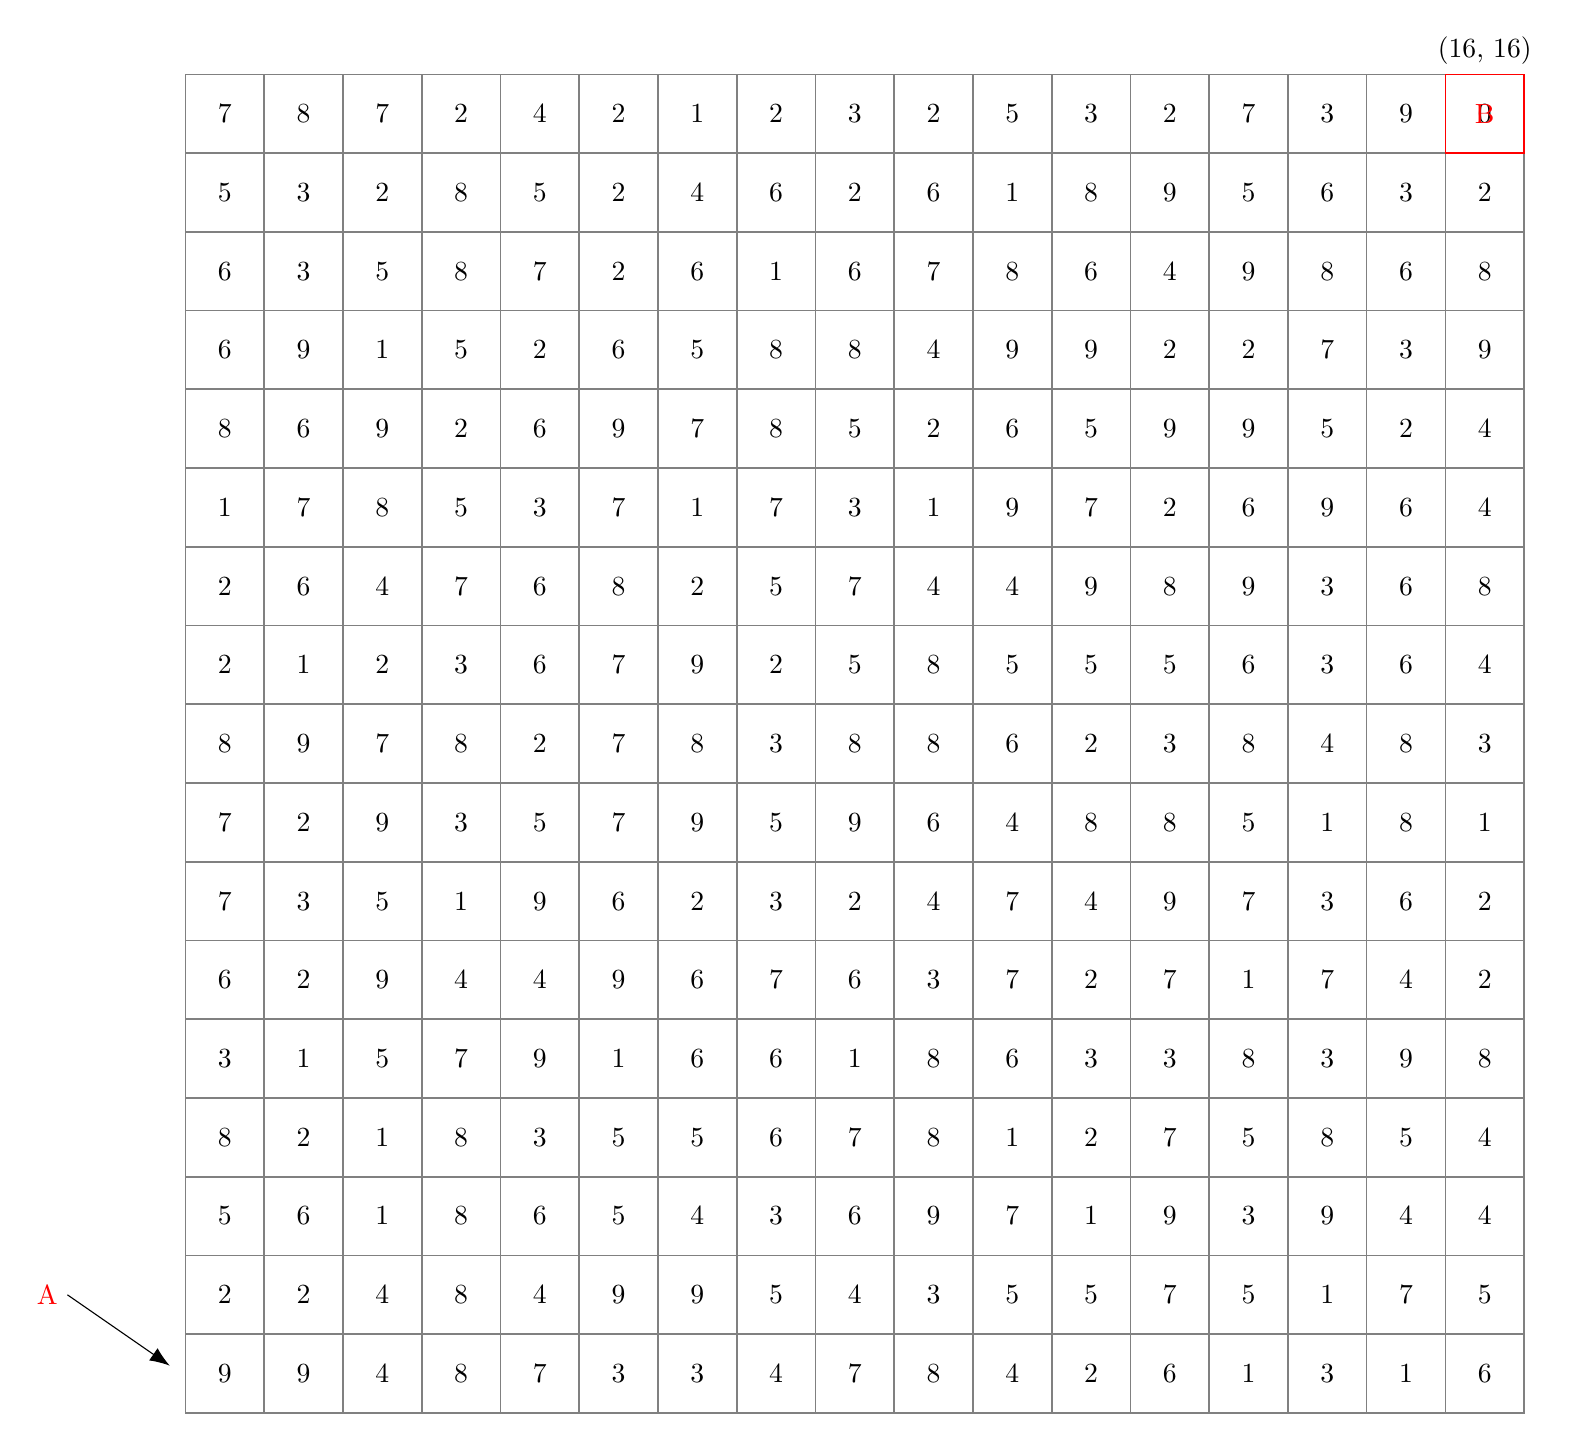
\begin{tikzpicture}[cell/.style = {rectangle,draw=gray,semithick,minimum size=1cm,outer sep=0mm}]
    \foreach \i [count=\j from 0] in {9,9,4,8,7,3,3,4,7,8,4,2,6,1,3,1,6} \node[cell] at (\j, 0) {$\i$};
    \foreach \i [count=\j from 0] in {2,2,4,8,4,9,9,5,4,3,5,5,7,5,1,7,5} \node[cell] at (\j, 1) {$\i$};
    \foreach \i [count=\j from 0] in {5,6,1,8,6,5,4,3,6,9,7,1,9,3,9,4,4} \node[cell] at (\j, 2) {$\i$};
    \foreach \i [count=\j from 0] in {8,2,1,8,3,5,5,6,7,8,1,2,7,5,8,5,4} \node[cell] at (\j, 3) {$\i$};
    \foreach \i [count=\j from 0] in {3,1,5,7,9,1,6,6,1,8,6,3,3,8,3,9,8} \node[cell] at (\j, 4) {$\i$};
    \foreach \i [count=\j from 0] in {6,2,9,4,4,9,6,7,6,3,7,2,7,1,7,4,2} \node[cell] at (\j, 5) {$\i$};
    \foreach \i [count=\j from 0] in {7,3,5,1,9,6,2,3,2,4,7,4,9,7,3,6,2} \node[cell] at (\j, 6) {$\i$};
    \foreach \i [count=\j from 0] in {7,2,9,3,5,7,9,5,9,6,4,8,8,5,1,8,1} \node[cell] at (\j, 7) {$\i$};
    \foreach \i [count=\j from 0] in {8,9,7,8,2,7,8,3,8,8,6,2,3,8,4,8,3} \node[cell] at (\j, 8) {$\i$};
    \foreach \i [count=\j from 0] in {2,1,2,3,6,7,9,2,5,8,5,5,5,6,3,6,4} \node[cell] at (\j, 9) {$\i$};
    \foreach \i [count=\j from 0] in {2,6,4,7,6,8,2,5,7,4,4,9,8,9,3,6,8} \node[cell] at (\j, 10) {$\i$};
    \foreach \i [count=\j from 0] in {1,7,8,5,3,7,1,7,3,1,9,7,2,6,9,6,4} \node[cell] at (\j, 11) {$\i$};
    \foreach \i [count=\j from 0] in {8,6,9,2,6,9,7,8,5,2,6,5,9,9,5,2,4} \node[cell] at (\j, 12) {$\i$};
    \foreach \i [count=\j from 0] in {6,9,1,5,2,6,5,8,8,4,9,9,2,2,7,3,9} \node[cell] at (\j, 13) {$\i$};
    \foreach \i [count=\j from 0] in {6,3,5,8,7,2,6,1,6,7,8,6,4,9,8,6,8} \node[cell] at (\j, 14) {$\i$};
    \foreach \i [count=\j from 0] in {5,3,2,8,5,2,4,6,2,6,1,8,9,5,6,3,2} \node[cell] at (\j, 15) {$\i$};
    \foreach \i [count=\j from 0] in {7,8,7,2,4,2,1,2,3,2,5,3,2,7,3,9,0} \node[cell] at (\j, 16) {$\i$};
\draw[{Latex[scale=1.5]}-] (-0.7, 0.1) -- (-2,1) node[left] {\textcolor{red}{A}};
\node[cell,red,label={(16, 16)}] at (16, 16) {B};
\end{tikzpicture}
}
\end{center}
\end{frame}

\begin{frame}[fragile]{問題1.3}{}
問題1.2を解くことで各ブロックのA地点からの最短移動時間が以下に示す配列Aに格納された。
AブロックからBブロックまでの最短経路を以下の形式で表示せよ。
\begin{quote}
(0,0) -> (?, ?) -> ... -> (16,16)
\end{quote}

\begin{center}
\scalebox{0.25}{
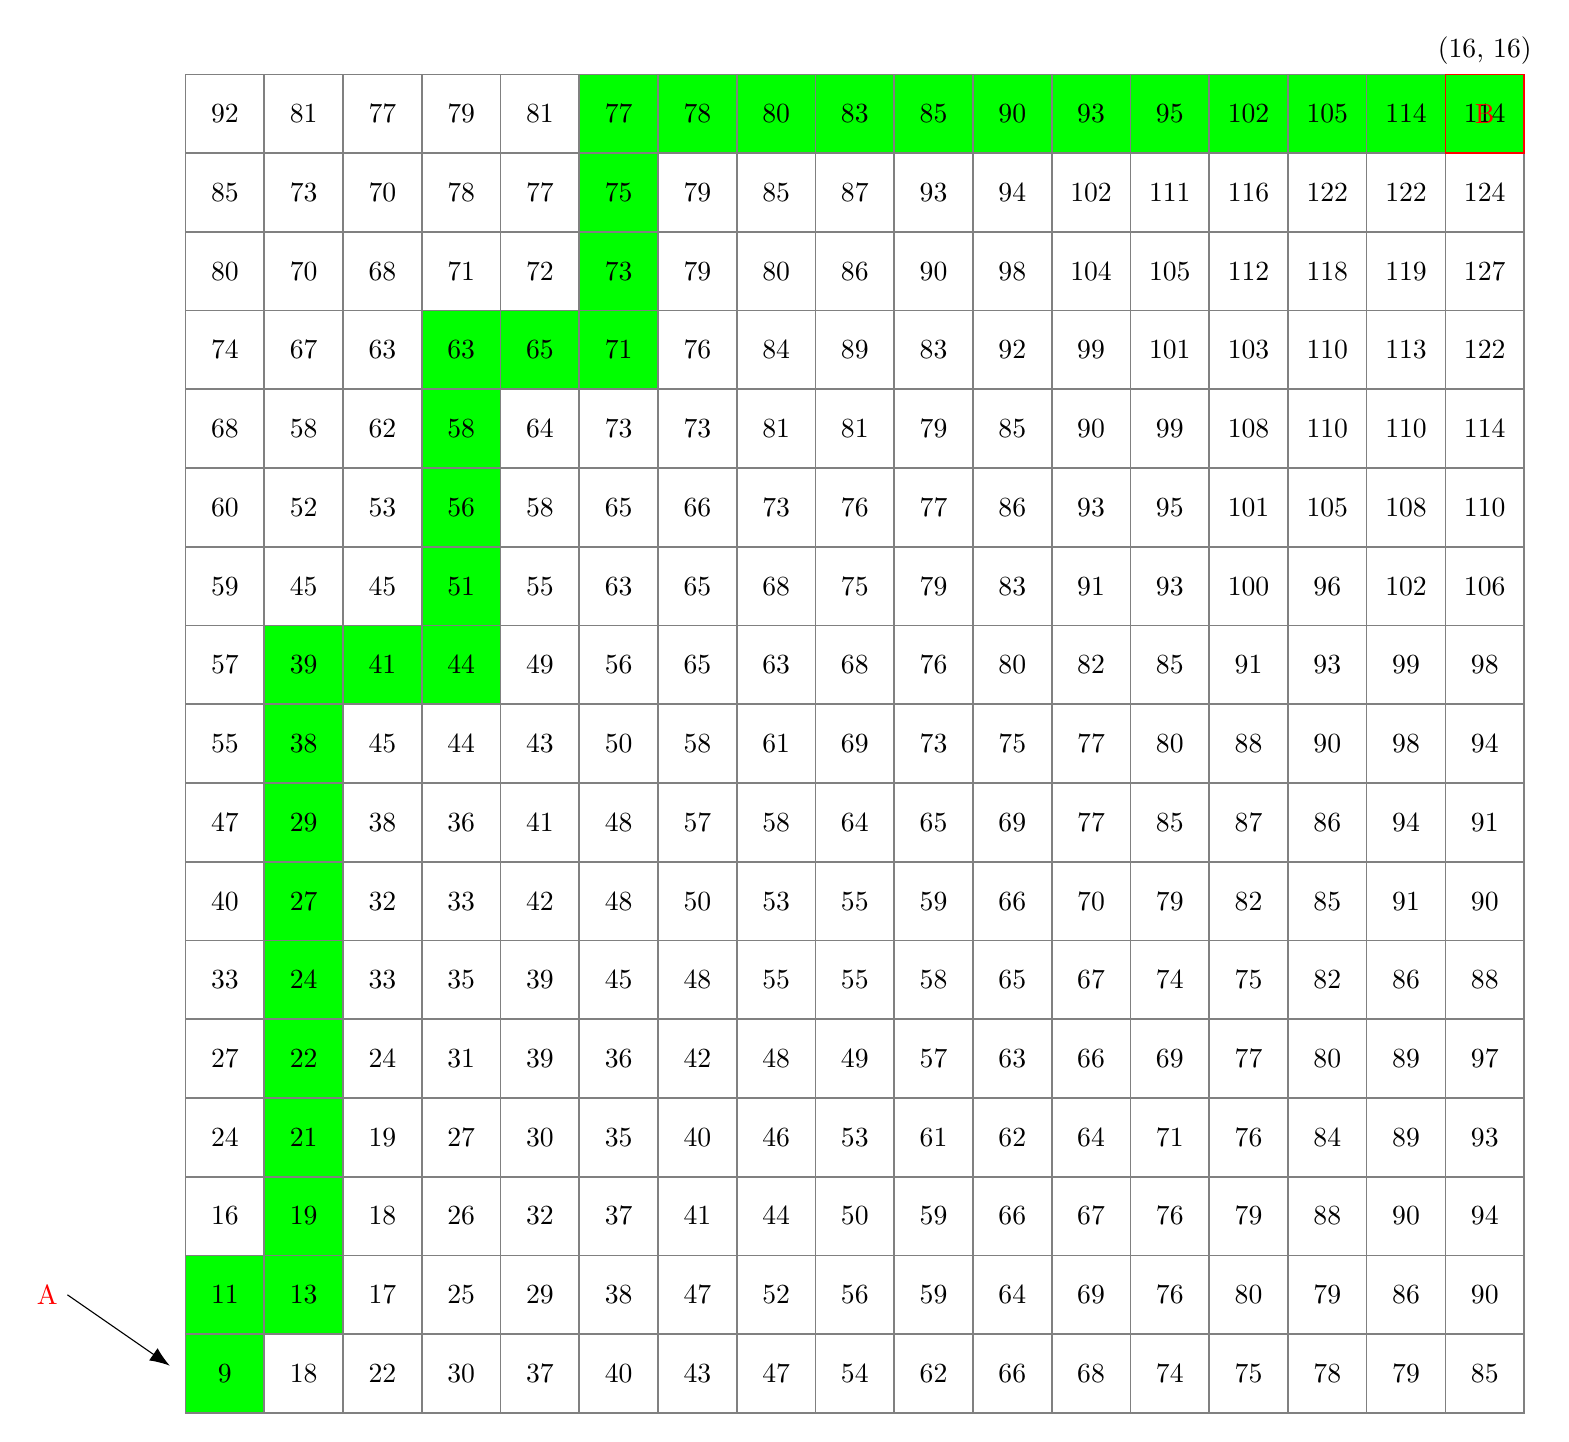
\begin{tikzpicture}[cell/.style = {rectangle,draw=gray,semithick,minimum size=1cm,outer sep=0mm}]
\visible<2>{    \foreach \j\i in { 0/0,1/0,1/1,2/1,3/1,4/1,5/1,6/1,7/1,8/1,9/1,9/2,9/3,10/3,11/3,12/3,13/3,13/4,13/5,14/5,15/5,16/5,16/6,16/7,16/8,16/9,16/10,16/11,16/12,16/13,16/14,16/15,16/16 }
 \node[cell,fill=green] at (\i, \j) {};}
\foreach \i [count=\j from 0] in {9,18,22,30,37,40,43,47,54,62,66,68,74,75,78,79,85} \node[cell] at (\j, 0) {$\i$};
\foreach \i [count=\j from 0] in {11,13,17,25,29,38,47,52,56,59,64,69,76,80,79,86,90} \node[cell] at (\j, 1) {$\i$};
\foreach \i [count=\j from 0] in {16,19,18,26,32,37,41,44,50,59,66,67,76,79,88,90,94} \node[cell] at (\j, 2) {$\i$};
\foreach \i [count=\j from 0] in {24,21,19,27,30,35,40,46,53,61,62,64,71,76,84,89,93} \node[cell] at (\j, 3) {$\i$};
\foreach \i [count=\j from 0] in {27,22,24,31,39,36,42,48,49,57,63,66,69,77,80,89,97} \node[cell] at (\j, 4) {$\i$};
\foreach \i [count=\j from 0] in {33,24,33,35,39,45,48,55,55,58,65,67,74,75,82,86,88} \node[cell] at (\j, 5) {$\i$};
\foreach \i [count=\j from 0] in {40,27,32,33,42,48,50,53,55,59,66,70,79,82,85,91,90} \node[cell] at (\j, 6) {$\i$};
\foreach \i [count=\j from 0] in {47,29,38,36,41,48,57,58,64,65,69,77,85,87,86,94,91} \node[cell] at (\j, 7) {$\i$};
\foreach \i [count=\j from 0] in {55,38,45,44,43,50,58,61,69,73,75,77,80,88,90,98,94} \node[cell] at (\j, 8) {$\i$};
\foreach \i [count=\j from 0] in {57,39,41,44,49,56,65,63,68,76,80,82,85,91,93,99,98} \node[cell] at (\j, 9) {$\i$};
\foreach \i [count=\j from 0] in {59,45,45,51,55,63,65,68,75,79,83,91,93,100,96,102,106} \node[cell] at (\j, 10) {$\i$};
\foreach \i [count=\j from 0] in {60,52,53,56,58,65,66,73,76,77,86,93,95,101,105,108,110} \node[cell] at (\j, 11) {$\i$};
\foreach \i [count=\j from 0] in {68,58,62,58,64,73,73,81,81,79,85,90,99,108,110,110,114} \node[cell] at (\j, 12) {$\i$};
\foreach \i [count=\j from 0] in {74,67,63,63,65,71,76,84,89,83,92,99,101,103,110,113,122} \node[cell] at (\j, 13) {$\i$};
\foreach \i [count=\j from 0] in {80,70,68,71,72,73,79,80,86,90,98,104,105,112,118,119,127} \node[cell] at (\j, 14) {$\i$};
\foreach \i [count=\j from 0] in {85,73,70,78,77,75,79,85,87,93,94,102,111,116,122,122,124} \node[cell] at (\j, 15) {$\i$};
\foreach \i [count=\j from 0] in {92,81,77,79,81,77,78,80,83,85,90,93,95,102,105,114,114} \node[cell] at (\j, 16) {$\i$};
\draw[{Latex[scale=1.5]}-] (-0.7, 0.1) -- (-2,1) node[left] {\textcolor{red}{A}};
\node[cell,red,label={(16, 16)}] at (16, 16) {B};
\end{tikzpicture}
}
\end{center}
\end{frame}

\begin{frame}[fragile]{問題2.0}{}
各点の重みが以下で与えられたとしてAからBへの最短距離を求めよ。各点は4近傍(4連結)である。

\begin{center}
\scalebox{0.3}{
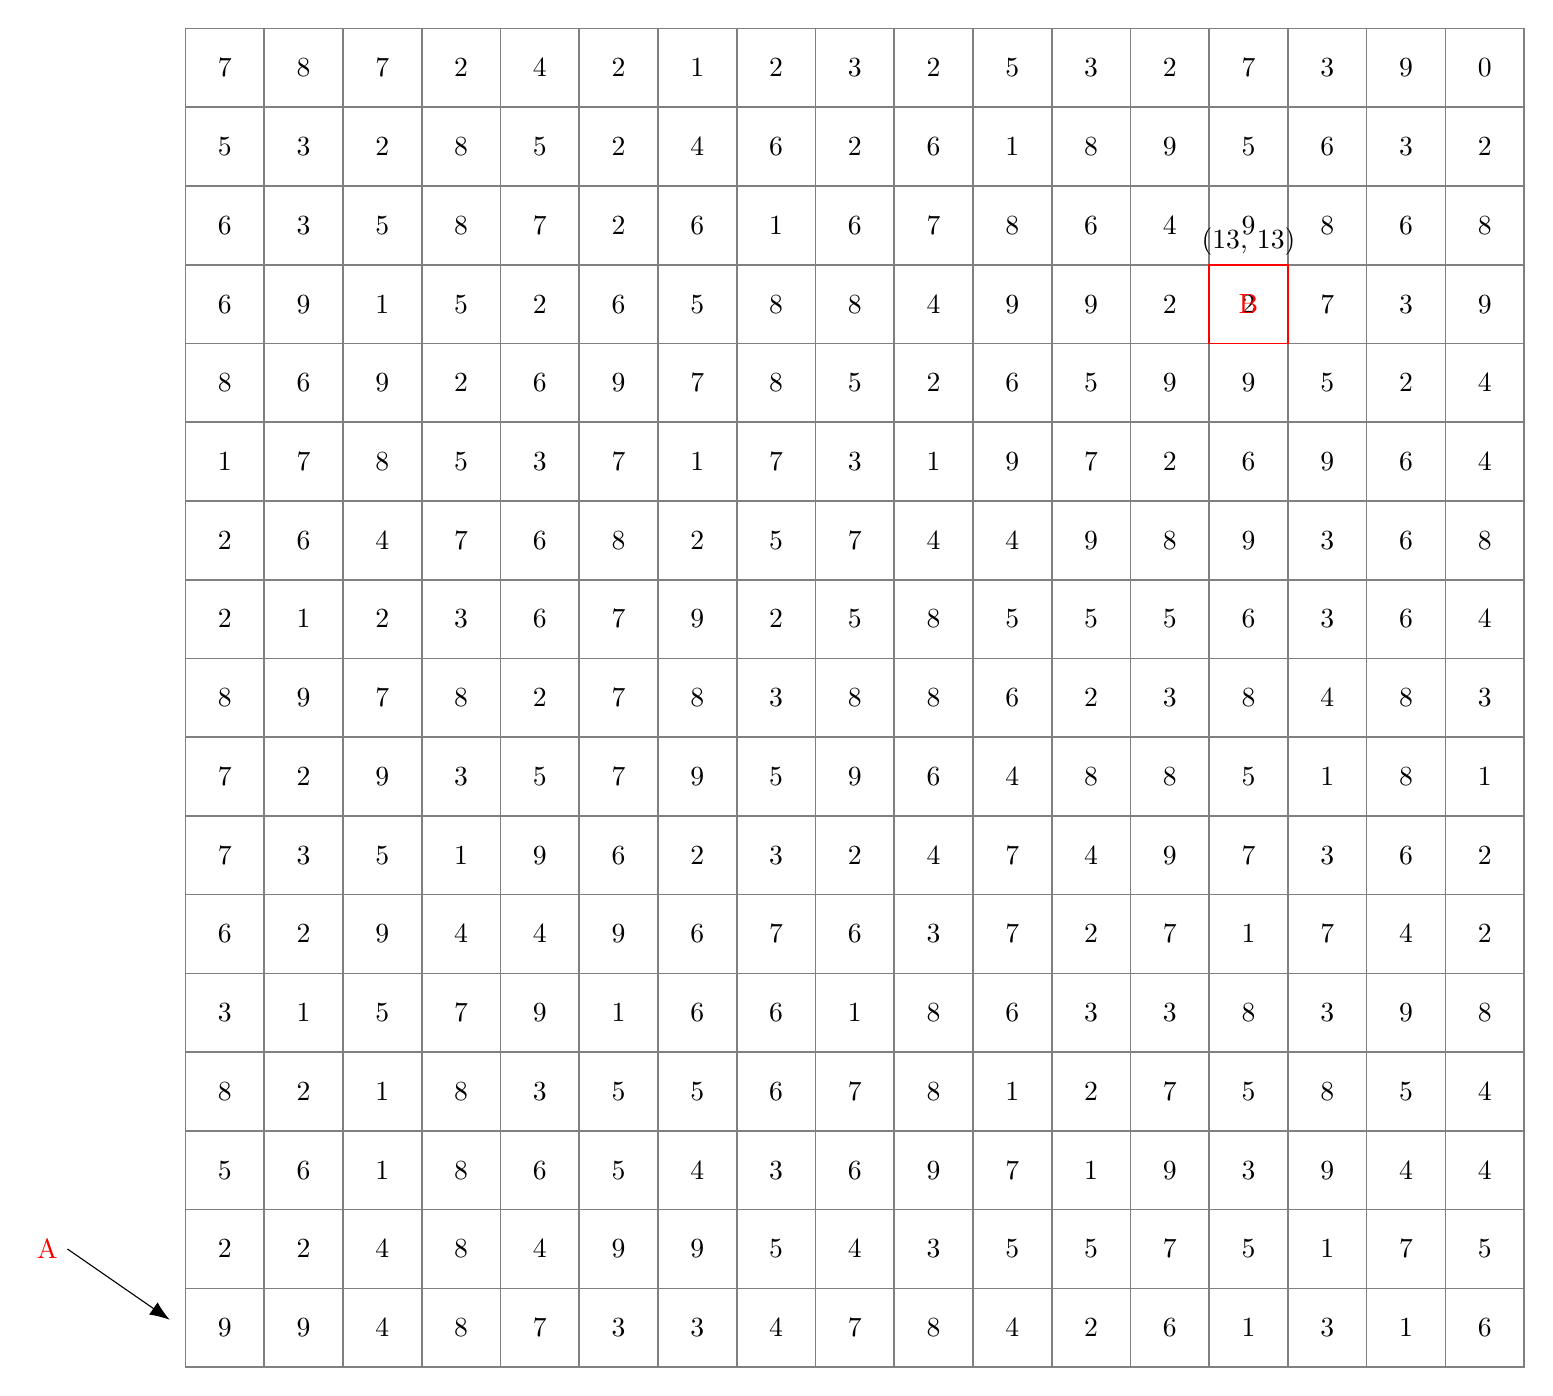
\begin{tikzpicture}[cell/.style = {rectangle,draw=gray,semithick,minimum size=1cm,outer sep=0mm}]
    \foreach \i [count=\j from 0] in {9,9,4,8,7,3,3,4,7,8,4,2,6,1,3,1,6} \node[cell] at (\j, 0) {$\i$};
    \foreach \i [count=\j from 0] in {2,2,4,8,4,9,9,5,4,3,5,5,7,5,1,7,5} \node[cell] at (\j, 1) {$\i$};
    \foreach \i [count=\j from 0] in {5,6,1,8,6,5,4,3,6,9,7,1,9,3,9,4,4} \node[cell] at (\j, 2) {$\i$};
    \foreach \i [count=\j from 0] in {8,2,1,8,3,5,5,6,7,8,1,2,7,5,8,5,4} \node[cell] at (\j, 3) {$\i$};
    \foreach \i [count=\j from 0] in {3,1,5,7,9,1,6,6,1,8,6,3,3,8,3,9,8} \node[cell] at (\j, 4) {$\i$};
    \foreach \i [count=\j from 0] in {6,2,9,4,4,9,6,7,6,3,7,2,7,1,7,4,2} \node[cell] at (\j, 5) {$\i$};
    \foreach \i [count=\j from 0] in {7,3,5,1,9,6,2,3,2,4,7,4,9,7,3,6,2} \node[cell] at (\j, 6) {$\i$};
    \foreach \i [count=\j from 0] in {7,2,9,3,5,7,9,5,9,6,4,8,8,5,1,8,1} \node[cell] at (\j, 7) {$\i$};
    \foreach \i [count=\j from 0] in {8,9,7,8,2,7,8,3,8,8,6,2,3,8,4,8,3} \node[cell] at (\j, 8) {$\i$};
    \foreach \i [count=\j from 0] in {2,1,2,3,6,7,9,2,5,8,5,5,5,6,3,6,4} \node[cell] at (\j, 9) {$\i$};
    \foreach \i [count=\j from 0] in {2,6,4,7,6,8,2,5,7,4,4,9,8,9,3,6,8} \node[cell] at (\j, 10) {$\i$};
    \foreach \i [count=\j from 0] in {1,7,8,5,3,7,1,7,3,1,9,7,2,6,9,6,4} \node[cell] at (\j, 11) {$\i$};
    \foreach \i [count=\j from 0] in {8,6,9,2,6,9,7,8,5,2,6,5,9,9,5,2,4} \node[cell] at (\j, 12) {$\i$};
    \foreach \i [count=\j from 0] in {6,9,1,5,2,6,5,8,8,4,9,9,2,2,7,3,9} \node[cell] at (\j, 13) {$\i$};
    \foreach \i [count=\j from 0] in {6,3,5,8,7,2,6,1,6,7,8,6,4,9,8,6,8} \node[cell] at (\j, 14) {$\i$};
    \foreach \i [count=\j from 0] in {5,3,2,8,5,2,4,6,2,6,1,8,9,5,6,3,2} \node[cell] at (\j, 15) {$\i$};
    \foreach \i [count=\j from 0] in {7,8,7,2,4,2,1,2,3,2,5,3,2,7,3,9,0} \node[cell] at (\j, 16) {$\i$};
\draw[{Latex[scale=1.5]}-] (-0.7, 0.1) -- (-2,1) node[left] {\textcolor{red}{A}};
\node[cell,red,label={(13, 13)}] at (13,13) {B};
\end{tikzpicture}
}
\end{center}
\end{frame}

\section{Extra puzzles}		%%%%%%%%
\subsection{}

\begin{frame}[fragile]{問題3}{Advent of Code: year 2020, day 10}
\begin{enumerate}\itemsep8pt
\item 与えられた数列は以下の条件を満たす数列に変換できるか
\begin{itemize}%\itemsep8pt
\item 全ての項は、直前の項より1、2、または3大きい
\end{itemize}
\begin{enumerate}%\itemsep8pt
\item 数列1:\{ 16, 10, 15, 5, 1, 11, 7, 19, 6, 12, 4 \}
\item 数列2:もっと長い(91項)ので次ページに掲載
\end{enumerate}
\item 所与の数列に対し以下の条件を満たす数列の個数を求めよ
\begin{itemize}%\itemsep8pt
\item その列中の全ての項は、直前の項より1、2、または3大きい
\item 与えられた全ての項を使わなくてよい
\item ただし、所与の数列の最小項は必ず使うこと
\item ただし、所与の数列の最大項は必ず使うこと
\end{itemize}
\begin{enumerate}%\itemsep8pt
\item 先の数列1
\begin{enumerate}%\itemsep8pt
\item 求める数列は1で始まらなければならない
\item 求める数列は19で終わらなければならない
\item 例えば\{ 1, 4, 5, 7, 10, 12, 15, 16, 19 \}は条件を満たす
\item 網羅すると8通りあることがわかるので答えは8
\end{enumerate}
\item (64bit CPU所有者のみ)次ページの数列2
\end{enumerate}
\end{enumerate}
\end{frame}

\begin{frame}[fragile]{数列2}{toa04-p3-seq2.txt}
95
43
114
118
2
124
120
127
140
21
66
103
102
132
136
93
59
131
32
9
20
141
94
109
143
142
65
73
27
83
133
104
60
110
89
29
78
49
76
16
34
17
105
98
15
106
4
57
1
67
71
14
92
39
68
125
113
115
26
33
61
45
46
11
99
7
25
130
42
3
10
54
44
139
50
8
58
86
64
77
35
79
72
36
80
126
28
123
119
51
22
\end{frame}

\end{document}
